\documentclass{article}

% Recommended, but optional, packages for figures and better typesetting:
\usepackage{microtype}
\usepackage{graphicx}
\usepackage{subfigure}
\usepackage{booktabs} % for professional tables

\usepackage{hyperref}
\usepackage{amsmath}
\usepackage{amssymb}

\newcommand{\theHalgorithm}{\arabic{algorithm}}

\usepackage[accepted]{icml2018}

\icmltitlerunning{Online Recommendation via Particle Thompson Sampling}

\begin{document}

\twocolumn[
\icmltitle{Online Recommendation via Particle Thompson Sampling}
\begin{icmlauthorlist}
\icmlauthor{Michael Alvarino}{equal}
\icmlauthor{Bharat Srikishan}{equal}
\icmlauthor{Colby Wise}{equal}
\end{icmlauthorlist}
\icmlaffiliation{equal}{Columbia University}
\vskip 0.3in
]

\begin{abstract}
Online recommendation is a difficult problem with many practical applications. A variety of
techniques exist to provide recommendations to users, but many require batch processing
and performance tradeoffs. We present a fast online recommendation system using Matrix
factorization, Thompson sampling, and particle filtering to provide cold start
movie recommendations to users. We also examine user preference drift for different
genres over time.
\end{abstract}

\section{Introduction}
Matrix factorization (MF) is a common tool for recommendation systems. While it provides useful
recommendations for users it requires a-priori knowledge of the set of users and items being
recommended. Real world use cases have online systems which must provide recommendations for
users that have no previous history (cold start users). Another problem in online systems is
the problem of user preference drift, as time progresses some users' preferences changes.

We combine the ideas of matrix factorization with bandit algorithms \cite{zhao2013interactive} to
build a model that solves these problems. Additionally, we use particle filtering to approximate
the posterior distribution.

\section{Model}

\subsection{Probabilistic Matrix Factorization}
We compute a low rank factorization of a ratings matrix $R$ where $R = UV^\top$. $U \in \mathbb{R}^{n \times k}$
and $V \in \mathbb{R}^{m \times k}$ are user and item latent matrices and $K$ is small. The probabilistic
model is:
\begin{gather*}
U_i \sim \mathcal{N}(0, \sigma_u^2 I_K) \\
V_i \sim \mathcal{N}(0, \sigma_v^2 I_K) \\
r_{ij} | U, V \sim \mathcal{N}(U_i^\top V_j, \sigma^2)
\end{gather*}
While this is a linear Gaussian model which has an analytically solvable conditional posterior, we use a
sequential Monte Carlo method to support our online inference. Specifically, we use a particle filter
based approach to approximate our posterior.

\subsection{Particle Thompson Sampling}
We use Thompson sampling while running our online linear bandit. This requires incremental updates
of the posterior $U$ and $V$. We implement a Rao-Blackwellized particle filter (RBPF) from
\cite{kawale2015efficient} based on the structure of our model. While iterating through the
ratings data for user $i$ and item $j$, we know that other user vectors $U_{-i}$ are independent
of this rating. Also, we know that other item vectors $V_{-j}$ are also unaffected. This
observation allows us to sample only $U_i$ and $V_j$, resulting in an efficient algorithm.

Each particle stores parameters $U, V, \sigma_U, \sigma_V$ and we sample $U_{i_t}|V, \sigma_U$
followed by $V_{j_t}|U, \sigma_v$:
\begin{gather*}
P(U_i | V, R^o, \sigma, \sigma_U) = P(U_i | V_{rts(i)}, R^o_{i, rts(i)}, \sigma_U, \sigma) \\
= \mathcal{N}(U_i | \mu^u_i, (\Lambda_i^u)^{-1}) \\
\text{where } \mu_i^u = \frac{1}{\sigma^2}(\Lambda_i^u)^{-1})\zeta_i^u \\
\Lambda_i^u = \frac{1}{\sigma^2} \sum_{j \in rts(i)} V_j V_j^{\top} + \frac{1}{\sigma_u^2}I_K \\
\zeta_i^u = \sum_{j \in rts(i)} r_{ij}^o V_j
\end{gather*}
Here $R^o$ are the observed ratings and $rts(i)$ is the set of items rated by user $i$.

\section{Experiments}

\subsection{Data}
We ran our experiments on the MovieLens 100k dataset. We only used the rating data for our
online recommendations, however we used the genre data in our evaluation of user preference
drift. We subtracted the mean rating from the data to center ratings at 0.

This dataset has 943 users, 1683 movies, and 100,000 ratings.

\section{Results}

\subsection{RMSE}
\begin{figure}[ht]

\begin{center}
\centerline{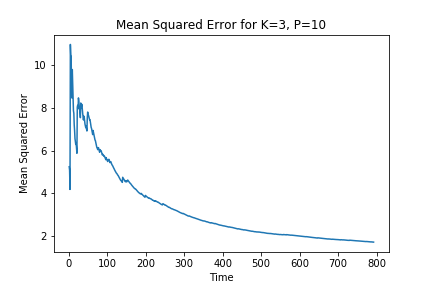
\includegraphics[width=\columnwidth]{TrainMSE}}
\caption{Training set mean squared error over time for K = 3 and 10 particles.}
\label{TrainMSE}
\end{center}
\vskip -0.2in
\end{figure}

We first examine mean squared error on the training set. As we see in Figure \ref{TrainMSE}, it decreases
over time as expected. The final MSE in this case is 1.721.

\begin{table}[ht]
\caption{Mean squared error statistics on the test set for various choices of K
(latent dimensionality) and P (number of particles)}
\label{sample-table}
\vskip 0.15in
\begin{center}
\begin{small}
\begin{sc}
\begin{tabular}{lcccc}
\toprule
(K, P) & Mean & Std Dev & Min & Max \\
\midrule
(2, 2)  & 2.924 & 0.355 & 2.512 & 3.585 \\
(2, 5)  & 2.981 & 0.387 & 2.552 & 3.711 \\
(3, 5)  & 2.540 & 0.182 & 2.408 & 2.900 \\
(3, 10) & 2.838 & 0.507 & 2.326 & 3.639 \\
(5, 2)  & 2.329 & 0.086 & 2.199 & 2.441 \\
(5, 10) & 2.367 & 0.088 & 2.251 & 2.519 \\
(5, 20) & 2.357 & 0.062 & 2.250 & 2.413 \\
\bottomrule
\end{tabular}
\end{sc}
\end{small}
\end{center}
\vskip -0.1in
\end{table}

\subsection{Cumulative Take Rate}

\subsection{Hyperparameter Cross Validation}

\subsection{User Preference Drift}

\section{Conclusion}

\nocite{kawale2015efficient}
\nocite{wang2017online}
\nocite{zhao2013interactive}
\nocite{cherkassky2013sequential}

\bibliographystyle{icml2018}
\bibliography{report}

\end{document}